\documentclass[11pt,a4paper]{article}

\usepackage[T1]{fontenc}
\usepackage[utf8]{inputenc}
\usepackage{lmodern}
\usepackage[margin=1in]{geometry}
\usepackage{microtype}
\usepackage{booktabs}
\usepackage{longtable}
\usepackage{array}
\usepackage{tabularx}
\usepackage{placeins}
\newcolumntype{Y}{>{\raggedright\arraybackslash}X}
\usepackage{enumitem}
\usepackage{xcolor}
\usepackage{caption}
\usepackage{fancyhdr}
\usepackage{hyperref}
\usepackage{tikz}
\usetikzlibrary{arrows.meta,positioning,shapes.geometric,fit,backgrounds}

\definecolor{qwpblue}{HTML}{1F3A5F}
\definecolor{qwpgray}{HTML}{F2F4F7}
\definecolor{qwpgreen}{HTML}{2E6B4F}
\definecolor{qwpred}{HTML}{8A2D2D}

\hypersetup{
  colorlinks=true,
  linkcolor=qwpblue,
  citecolor=qwpblue,
  urlcolor=qwpblue,
  pdftitle={qWp: A Versioned Hash-Based Signature Family with Exhaustive Local Verification},
  pdfauthor={qWp Project},
  pdfsubject={White paper, long version},
  pdfkeywords={hash-based signatures, post-quantum, verification, safe Rust, formal methods}
}

\pagestyle{fancy}
\fancyhf{}
\fancyhead[L]{\small qWp White Paper}
\fancyhead[R]{\small Version 1.0}
\fancyfoot[C]{\thepage}
\renewcommand{\headrulewidth}{0.4pt}

\setlength{\parindent}{1.2em}
\setlength{\parskip}{0.35em}
\linespread{1.12}
\setlist[itemize]{topsep=0.3em,itemsep=0.15em,parsep=0.1em}
\setlist[enumerate]{topsep=0.3em,itemsep=0.15em,parsep=0.1em}

\newcommand{\qwp}{\textsc{qWp}}
\newcommand{\tool}[1]{\textsf{#1}}
\newcommand{\doc}[1]{\emph{#1}}

\title{
  \vspace*{1.2cm}
  {\Huge\bfseries \qwp}\\[0.35cm]
  {\LARGE A Versioned Hash-Based Signature Family\\[0.15cm]
  with Exhaustive Local Verification}\\[0.9cm]
  {\Large White Paper --- Long Version}\\[0.5cm]
  {\large Design, security arguments, code standard, engineering,\\
  verification methodology, results, and assurance limits}
  \vspace{1.0cm}
}
\author{\large \qwp{} Project}
\date{November 2026}

\begin{document}

\maketitle
\thispagestyle{empty}

\begin{abstract}
\noindent
\qwp{} is a versioned family of hash-based signature schemes and verification
profiles built around a deliberately narrow engineering doctrine: no external
runtime dependencies, no unsafe code, a no-standard-library cryptographic core,
explicit version separation, and evidence-first release gates. The family spans
stateful one-time-signature trees (QHS-1, QHS-2, QHS-3, QHS-3.1), stateless
hypertree and forest constructions (QHS-4, QHS-4.1, QHS-4.2), a 512-bit-margin
stateful profile (QHS-5), a transcript-bound hybrid with an in-tree classical
component (QHS-6), and a verifier-only embedded profile (QHS-E). This white
paper presents the design rationale, threat model, construction family,
security arguments, implementation discipline, the full code standard, the
verification and attack methodology, and the measured evidence. The evidence
includes 308 release tests, 20 attack groups, exhaustive single-bit mutation of
every signature byte, Kani model checking, Creusot deductive verification of
the digit and checksum arithmetic, AORAI temporal analysis of the verification
order, libFuzzer and custom fuzzing, property-based testing, Loom concurrency
modeling, dudect timing analysis, Miri undefined-behavior checking, coverage,
mutation testing, code-size and stack measurement, and per-version one-hour
soaks. QHS-E passed a one-hour soak with 28,798,916 iterations and zero panics
and is tagged \emph{qhse-rc1}. A 72-hour all-version soak runner is prepared but
has not yet been run. The paper closes with an explicit list of assurance gaps,
chief among them the absence of an independent external audit and a certified
compiler path.
\end{abstract}

\newpage
\tableofcontents
\listoftables
\listoffigures
\newpage

\section{Executive Summary}

\qwp{} began as an investigation into a non-standard topological signature
idea and ended as a disciplined, versioned hash-based signature family. The
original construction was rejected after a structural break was identified.
The project then adopted a conservative hash-based design space, wrote down a
threat model and a release rule, and implemented each version as an independent
artifact with its own architecture decision record, proof, format, domain
contexts, tests, attack harness, fuzz coverage, timing, and soak.

The central engineering choice is \emph{zero external runtime dependencies}.
The production workspace contains only first-party crates and uses the Rust
core and standard libraries. The cryptographic core is no-standard-library,
allocation-free where required, and every crate forbids unsafe code. This makes
the trusted computing base small enough to inspect, but it also means that the
hash function, the classical signature component, the command-line interface,
and the test harnesses are all first-party code. The project compensates with
an unusually broad local verification programme rather than with external
libraries.

The family is organized around six design axes: stateful versus stateless
signing; signatures per key; signature size; signing latency; quantum margin;
and verifier profile. QHS-1 is the speed-first stateful profile. QHS-2 is the
compact stateful profile. QHS-3 raises capacity to 4,096 signatures per key;
QHS-3.1 keeps the same keys and signatures and adds a tree cache for fast
signing. QHS-4 introduces a stateless hypertree and forest construction;
QHS-4.1 is its parallel fast-signing profile; QHS-4.2 is a compact stateless
parameter set. QHS-5 raises the hash width and the security margin to 256-bit
classical and approximately 128-bit quantum. QHS-6 composes QHS-5 with an
in-tree Ed25519 implementation over a key-and-message transcript. QHS-E is a
verifier-only profile of QHS-1, QHS-2, QHS-3, and QHS-3.1 for bootloaders and
constrained microcontrollers.

The verification programme is layered. Unit, integration, and known-answer
tests establish functional behavior. Differential tests compare independent
verifier implementations. Property-based tests explore invariants. Two fuzzing
approaches, a deterministic in-house driver and a libFuzzer target, search for
panics and parser edge cases. Kani proves parser and bounds properties. Creusot
proves the arithmetic of the digit, checksum, and Merkle-index model. AORAI
checks the temporal order of the verification stages on a C model. Loom models
the parallel chunk-and-join protocol. dudect measures timing separation.
cargo-show-asm inspects generated assembly. Miri checks undefined behavior.
Coverage, mutation testing, code-size measurement, stack measurement, timing,
and one-hour soaks complete the evidence.

The results are strong for a local, first-party project but are not a
substitute for external review. The production gap register is empty, the
research backlog remains separate, and the release rule has been followed for
each version. QHS-E is the newest release candidate. It passed a one-hour soak
with 28,798,916 iterations and zero panics, has a measured peak verifier stack
of about six kilobytes, and is tagged \emph{qhse-rc1}. The remaining assurance
gaps are external audit, a certified compiler path, complete path coverage,
full formal verification of the hash-based verifier, hardware cycle
measurement, and the residual state-guard limitation at counter zero.

\section{Scope, Contributions, and Non-Claims}

\subsection{Scope}

This paper covers the production signature family, the host-side tooling, the
embedded verifier profile, the code standard, and the verification evidence
through the current local snapshot. It describes what was built, why each
choice was made, how the implementations are checked, and what the measurements
show. It also states what is not claimed.

\subsection{Contributions}

The main contributions are:

\begin{enumerate}
  \item A versioned hash-based signature family with explicit parameter,
  format, domain, cache, and state separation.
  \item A zero-dependency, safe-Rust implementation of the hash function, the
  classical component, the signature schemes, and the verification tooling.
  \item A strict code standard with a documented crate classification and a
  runnable audit.
  \item A layered local verification methodology combining testing, fuzzing,
  model checking, deductive verification, temporal analysis, concurrency
  modeling, timing analysis, assembly inspection, undefined-behavior checking,
  coverage, mutation testing, and soak testing.
  \item An exhaustive single-bit mutation study of every signature format and
  structural attacks that repair the unkeyed format checksum before verifying.
  \item A verifier-only embedded profile with measured code size, stack use,
  timing, and differential equivalence to the base verifiers.
  \item A public record of the defects found during the work and the fixes
  applied, including public-key canonicalization, state-guard fail-closed
  behavior, and embedded-component header validation.
\end{enumerate}

\subsection{Non-claims}

The project does not claim:

\begin{itemize}
  \item that it is a standard, or that it is compliant with a standards body;
  \item that it has been independently audited;
  \item that it has been built with a certified compiler;
  \item that every line of every crate is covered by a test;
  \item that the formal artifacts prove the full Rust verifier and the hash
  function end to end;
  \item that host timing is a hardware cycle measurement;
  \item that the state guard is a hardware counter or a trusted external
  monotonic state;
  \item that the 72-hour soak has already passed.
\end{itemize}

These non-claims are not footnotes. They define the boundary between local
evidence and deployment assurance.

\section{Threat Model and Design Doctrine}

\subsection{Adversary model}

The adversary is assumed to be able to choose messages, public keys,
signatures, cache files, state files, and command-line inputs. The adversary
may attempt to forge signatures, confuse versions, substitute components, roll
back state, corrupt caches, exploit parser edge cases, induce panics, or learn
secret-dependent timing. The adversary is not assumed to break the underlying
hash function or the classical component by cryptanalysis. The adversary may
be classical or quantum; the security targets are stated per version.

The signer is assumed to be a single writer for stateful versions. If the
signer can be cloned, restored, or rolled back together with its state, the
one-time-signature guarantee can be lost. The project mitigates this with an
atomic key store, a keyed state guard, a lock file, and a strict signing order,
but it cannot create a trusted monotonic counter out of local files alone.

\subsection{Stateful signing}

Stateful hash-based signatures consume a leaf per signature. Reusing a leaf
with two different messages breaks the one-time-signature security argument.
The implementation therefore persists the advanced counter before releasing
the signature, refuses a key whose guard counter is ahead of the key counter,
and refuses a corrupt or missing guard for an advanced key. The residual
limitation is that deleting the guard and rolling the key counter back to zero
is indistinguishable from a fresh key without external trusted state.

\subsection{Stateless signing}

Stateless versions avoid the counter entirely. The signer may be cloned and
run concurrently. The price is a larger signature, a more complex hypertree and
forest construction, and a different security argument. QHS-4, QHS-4.1, and
QHS-4.2 are the stateless members of the family.

\subsection{Design doctrine}

The doctrine has five parts:

\begin{enumerate}
  \item \textbf{Zero external runtime dependencies.} The production workspace
  uses only first-party crates and the Rust core and standard libraries.
  \item \textbf{No unsafe code.} Every crate forbids unsafe code. There are no
  raw pointers, no manual memory management, and no foreign function calls in
  first-party source.
  \item \textbf{No-standard-library cryptographic core.} The production crypto
  crates do not require the standard library, the heap, threads, or the
  operating system. Host adapters provide entropy, files, threads, and
  reporting.
  \item \textbf{Explicit version separation.} Every version has its own
  header, domain contexts, signature size, key layout, cache layout, and
  release gate. A version is never silently extended.
  \item \textbf{Evidence-first release.} A version is not called ready until the
  proof, formats, tests, attacks, fuzzing, timing, mutation, coverage, and soak
  evidence exist.
\end{enumerate}

The doctrine is deliberately conservative. It accepts more first-party code in
exchange for a small, inspectable dependency graph. It accepts slower
development in exchange for version separation. It accepts a larger local
verification burden in exchange for not trusting opaque libraries.

\section{System Architecture}

\subsection{Crate topology}

The workspace is a set of small crates with one-directional dependencies. The
cryptographic core is separated from the host adapters. The verifier profile
depends on the core and hash crates but not on the signing crate. The attack,
benchmark, test, and proof crates depend on the production crates but are not
part of the production trust boundary.

\begin{figure}[ht]
\centering
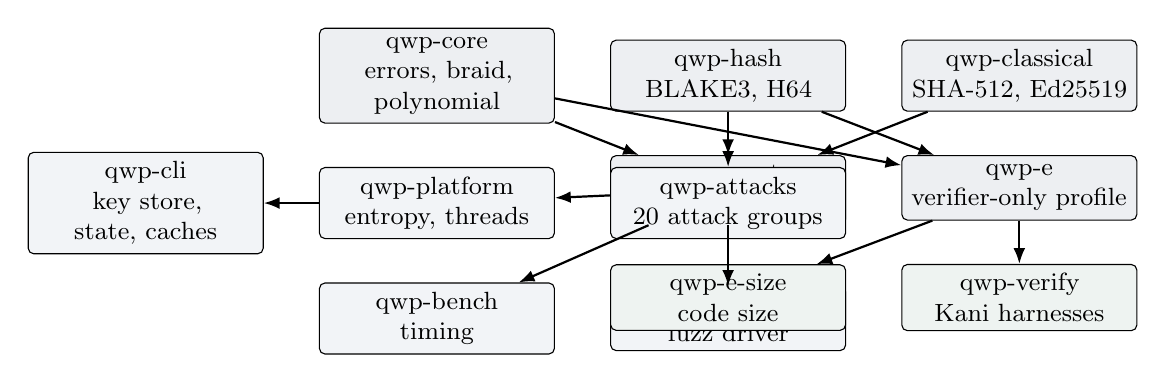
\begin{tikzpicture}[
  node distance=0.55cm and 0.7cm,
  box/.style={draw, rounded corners=2pt, align=center, minimum height=0.75cm, text width=2.75cm, font=\small},
  core/.style={box, fill=qwpblue!8},
  host/.style={box, fill=qwpgray},
  proof/.style={box, fill=qwpgreen!8},
  arrow/.style={-{Latex[length=2mm]}, thick}
]
\node[core] (core) {qwp-core\\errors, braid, polynomial};
\node[core, right=of core] (hash) {qwp-hash\\BLAKE3, H64};
\node[core, right=of hash] (classical) {qwp-classical\\SHA-512, Ed25519};
\node[core, below=of hash] (crypto) {qwp-crypto\\QHS family};
\node[core, below=of classical] (e) {qwp-e\\verifier-only profile};
\node[host, below=of core] (platform) {qwp-platform\\entropy, threads};
\node[host, left=of platform] (cli) {qwp-cli\\key store, state, caches};
\node[host, right=of platform] (attacks) {qwp-attacks\\20 attack groups};
\node[host, below=of platform] (bench) {qwp-bench\\timing};
\node[host, right=of bench] (tests) {qwp-tests\\fuzz driver};
\node[proof, below=of e] (verify) {qwp-verify\\Kani harnesses};
\node[proof, left=of verify] (size) {qwp-e-size\\code size};
\draw[arrow] (core) -- (crypto);
\draw[arrow] (hash) -- (crypto);
\draw[arrow] (classical) -- (crypto);
\draw[arrow] (core) -- (e);
\draw[arrow] (hash) -- (e);
\draw[arrow] (crypto) -- (platform);
\draw[arrow] (platform) -- (cli);
\draw[arrow] (crypto) -- (attacks);
\draw[arrow] (crypto) -- (bench);
\draw[arrow] (crypto) -- (tests);
\draw[arrow] (e) -- (verify);
\draw[arrow] (e) -- (size);
\end{tikzpicture}
\caption{Simplified crate topology. The production crypto core is separated
from host adapters, attacks, benchmarks, tests, and proof harnesses. Arrows
show the main dependency direction; not every transitive edge is drawn.}
\label{fig:topology}
\end{figure}

\subsection{Cryptographic core}

The cryptographic core consists of five production crates. The core crate
provides errors, the legacy braid and polynomial containers, validation, and
serialization. The hash crate provides the in-tree BLAKE3 implementation,
including keyed hashing, derive-key contexts, streaming, and the 512-bit H64
mode. The classical crate provides SHA-512 and Ed25519 for the hybrid version.
The signature crate implements the QHS family and the legacy containers. The
embedded crate implements the verifier-only profile.

\subsection{Host adapters and tooling}

The platform crate provides safe entropy from the operating system and
parallel leaf and tree generation on the host. The command-line crate provides
key generation, signing, verification, caches, the state guard, and self-tests.
The attack crate contains adversarial harnesses. The benchmark crate contains
timing harnesses. The test crate contains the deterministic fuzz driver. The
proof crate contains Kani harnesses. The size crate is a standalone static
library probe for embedded code-size measurement.

\subsection{Formats and version separation}

Every public key, private key, signature, cache, and state file has a fixed
layout and a version header. The header is checked at parse time and again at
verification time. Domain contexts include the version name, so a signature
computed for one version does not verify under another even if the byte lengths
coincide. The verifier profile uses the base-version contexts rather than new
ones, because it is an implementation profile, not a new signature format.

\section{The \qwp{} Version Family}

\subsection{Common construction}

The stateful members use a Winternitz one-time signature over hash chains, a
Merkle tree over one-time public keys, and a signature that reveals one chain
value per digit plus the authentication path. The message is hashed with a
domain-separated derive-key context and encoded as digits. A small checksum
over the digits protects against some classes of digit manipulation, but the
checksum is not an authenticator; the cryptographic binding comes from the
one-time signature and the Merkle path.

The stateless members use a forest of few-time signatures to compress the
message into a set of leaf indices, followed by a multi-layer hypertree. The
hypertree lets the signer authenticate a fresh subtree at each layer without a
global counter. The trade-off is a larger signature and a more involved
security argument.

The hybrid member composes a stateful 512-bit-margin signature with a classical
signature over the same key-and-message transcript. Verification requires both
components. The transcript includes both public keys and the message, which
prevents component mixing across messages or keys.

\subsection{QHS-1: speed-first stateful}

QHS-1 is the first production version. It uses 67 hash chains of length 15,
a Merkle tree of height 8, 64-byte public and private keys, and a 2,408-byte
signature. It provides 256 signatures per key. The message encoding uses
hexadecimal digits plus a three-digit checksum. Key generation is about ten to
thirteen milliseconds on the host, signing is about two to three tenths of a
millisecond, and verification is about one tenth of a millisecond. The version
is intended for offline signing where speed and simplicity matter.

\subsection{QHS-2: compact stateful}

QHS-2 keeps the height-8 tree and 256-signature capacity but uses 45 chains of
length 63 and a base-64 message encoding. The signature shrinks to 1,704 bytes.
Key generation is about 27 to 28 milliseconds, signing is about half a
millisecond, and verification is about four tenths of a millisecond. The
compact signature makes QHS-2 suitable for firmware and release signing where
bandwidth or storage is constrained.

\subsection{QHS-3 and QHS-3.1: high-capacity stateful}

QHS-3 keeps the QHS-2 one-time signature parameters and raises the Merkle tree
to height 12. The capacity becomes 4,096 signatures per key, the signature is
1,832 bytes, and the authentication path grows by 128 bytes. Key generation is
about four tenths of a second, signing is about 1.6 to 1.7 milliseconds, and
verification is about 0.39 milliseconds. QHS-3.1 is a profile of QHS-3 with a
tree cache. Keys, signatures, known-answer tests, and the proof are identical;
signing drops to about 0.35 to 0.36 milliseconds. The cache is 262,180 bytes
and contains public tree data only.

\subsection{QHS-4 and QHS-4.1: stateless hypertree and forest}

QHS-4 is the first stateless version. It uses a forest of few-time signatures
with 16 trees of height 8 and an eight-layer hypertree with subtree height 8,
for a total height of 64. The public and private keys are 68 bytes, the
signature is 18,216 bytes, and there is no counter, cache, or state guard.
Key generation is about one tenth of a second, sequential signing is about
0.81 seconds, and verification is about 1.6 milliseconds. The design targets
128-bit classical security and at least 64-bit quantum security for up to about
one million signatures. QHS-4.1 keeps the same keys, signatures, and proof and
parallelizes tree and forest generation. Signing drops to about 0.11 seconds,
roughly seven times faster, with byte-identical output.

\subsection{QHS-4.2: compact stateless}

QHS-4.2 is a compact stateless parameter set. It uses 34 chains of length 255,
a seven-layer hypertree with total height 56, and 17 forest trees of height 8.
The signature shrinks to 14,344 bytes, about twenty-one percent smaller than
QHS-4. Key generation is about 0.30 seconds, parallel signing is about 0.27
seconds, and verification is about 4.0 milliseconds. The security target is the
same 128-bit classical and at least 64-bit quantum target for up to about one
million signatures.

\subsection{QHS-5: 512-bit margin}

QHS-5 is the 512-bit-margin stateful profile. It uses a 512-bit hash mode,
89 chains of length 63, a height-8 tree, 72-byte keys, and a 6,216-byte
signature. It provides 256 signatures per key and targets 256-bit classical and
approximately 128-bit quantum security. Parallel key generation is about
0.09 seconds, cached signing is about 1.5 milliseconds, uncached signing is
about 0.62 seconds, and verification is about 1.2 milliseconds. The leaf cache
is 16,452 bytes and the state guard is 38 bytes.

\subsection{QHS-6: transcript-bound hybrid}

QHS-6 composes QHS-5 with Ed25519. The public key is 108 bytes, the signature
is 6,284 bytes, and the capacity is 256 signatures per key. Both components
sign a transcript that includes the QHS-5 public key, the Ed25519 public key,
and the message. Verification requires both signatures. The hybrid is intended
for migration and compliance settings where a classical component is required.
The in-tree Ed25519 implementation passes the RFC 8032 test vectors. Hybrid key
generation is about 0.09 seconds, cached signing is about 2.0 milliseconds, and
verification is about 1.5 milliseconds.

\subsection{QHS-E: embedded verifier profile}

QHS-E is not a new signature. It is a verifier-only profile of QHS-1, QHS-2,
QHS-3, and QHS-3.1. It accepts the same public keys and signatures, uses the
same headers, digits, chains, contexts, leaf and node hashing, and checksum, and
returns the same accept or reject decision as the base verifier. It has no key
generation, signing, cache, or state guard. It is no-standard-library,
allocation-free, and forbids unsafe code. The measured code size is 12,771
bytes on the thumbv7em target and 14,247 bytes on the riscv32imac target for
all four entry points. The measured peak verifier stack is about six kilobytes,
driven by the BLAKE3 hasher; the shared verifier frame itself is about 256 to
264 bytes. Host verification is about 0.14 milliseconds for QHS-1, 0.32
milliseconds for QHS-2, and 0.39 milliseconds for QHS-3 and QHS-3.1.

\subsection{Parameter and performance matrix}

\begin{table}[ht]
\centering
\caption{Version parameters. Numbers are measured on the development host and
are not hardware cycle claims.}
\label{tab:versions}
\footnotesize
\begin{tabularx}{\textwidth}{@{}p{1.35cm}p{4.6cm}c c Y@{}}
\toprule
Version & Construction & Stateful & Sigs/key & Signature\\
\midrule
QHS-1 & 67 by 15 chains, height 8 & Yes & 256 & 2,408 B\\
QHS-2 & 45 by 63 chains, height 8 & Yes & 256 & 1,704 B\\
QHS-3 & 45 by 63 chains, height 12 & Yes & 4,096 & 1,832 B\\
QHS-3.1 & QHS-3 with tree cache & Yes & 4,096 & 1,832 B\\
QHS-4 & 8-layer hypertree, forest 16 by 8 & No & about 1,000,000 & 18,216 B\\
QHS-4.1 & QHS-4 with parallel trees & No & about 1,000,000 & 18,216 B\\
QHS-4.2 & 7-layer hypertree, forest 17 by 8 & No & about 1,000,000 & 14,344 B\\
QHS-5 & 512-bit hash, 89 by 63 chains & Yes & 256 & 6,216 B\\
QHS-6 & QHS-5 plus Ed25519 hybrid & Yes & 256 & 6,284 B\\
QHS-E & verifier-only QHS-1/2/3/3.1 & No & not applicable & same as base\\
\bottomrule
\end{tabularx}
\end{table}
\FloatBarrier

\begin{table}[ht]
\centering
\caption{Host performance. Measurements are not hardware cycle claims.}
\label{tab:performance}
\footnotesize
\begin{tabularx}{\textwidth}{@{}l c c Y@{}}
\toprule
Version & Keygen & Sign & Verify\\
\midrule
QHS-1 & 10--13 ms & 0.21--0.33 ms & 0.14 ms\\
QHS-2 & 27--28 ms & 0.46--0.61 ms & 0.41 ms\\
QHS-3 & 0.40--0.44 s & 1.60--1.70 ms & 0.39 ms\\
QHS-3.1 & 0.40--0.41 s & 0.35--0.36 ms & 0.39 ms\\
QHS-4 & 0.10 s & 0.81 s & 1.6 ms\\
QHS-4.1 & 0.10 s & 0.11 s & 1.6 ms\\
QHS-4.2 & 0.30 s & 0.27 s & 4.0 ms\\
QHS-5 & 0.09 s parallel & 1.5 ms cached & 1.2 ms\\
QHS-6 & 0.09 s & 2.0 ms cached & 1.5 ms\\
QHS-E & not applicable & not applicable & 0.14--0.39 ms\\
\bottomrule
\end{tabularx}
\end{table}
\FloatBarrier

\begin{table}[ht]
\centering
\caption{Stated security targets. The targets are design claims supported by
the internal proofs and evidence; they are not an external certification.}
\label{tab:security}
\footnotesize
\setlength{\tabcolsep}{4pt}
\begin{tabularx}{\textwidth}{@{}l l l Y@{}}
\toprule
Version & Classical target & Quantum target & Notes\\
\midrule
QHS-1/2/3/3.1 & 128-bit & 64-bit baseline & Stateful; single-writer counter required.\\
QHS-4/4.1/4.2 & 128-bit & at least 64-bit for up to about one million signatures & Stateless; larger signatures.\\
QHS-5 & 256-bit & approximately 128-bit & 512-bit hash margin.\\
QHS-6 & QHS-5 or Ed25519 & QHS-5 or Ed25519 & Hybrid; secure if either component is secure.\\
QHS-E & same as base & same as base & Verifier-only profile; no new assumption.\\
\bottomrule
\end{tabularx}
\end{table}
\FloatBarrier

\section{Security Arguments}

\subsection{Stateful reductions}

The stateful versions reduce existential unforgeability under chosen-message
attack to the collision and preimage resistance of the underlying hash
function, together with the one-time-signature and Merkle-tree arguments. The
proof is written in prose and checked against the implementation: the message
digits, chain lengths, chain counts, leaf hashing, node hashing, domain
contexts, and checksum range must match the proof. The known-answer tests and
differential tests are the implementation-level check that the proof and code
agree.

\subsection{Leaf-reuse bounds}

A stateful key is a finite resource. The security argument assumes that each
leaf is used at most once. The implementation enforces this with a persisted
counter and a keyed state guard. The guard is not a hardware counter. If the
key and guard are restored together, the local software cannot detect the
rollback. This is stated as a deployment limitation, not hidden.

\subsection{Stateless hypertree and forest}

The stateless versions use a forest of few-time signatures to derive a set of
leaf indices, then a multi-layer hypertree to authenticate the selected leaves.
The security argument accounts for the number of signatures, the forest
parameters, the subtree height, and the number of layers. QHS-4 and QHS-4.2
target 128-bit classical security and at least 64-bit quantum security for up
to about one million signatures. The proof is in the version documents and is
checked by known-answer tests, attacks, fuzzing, and timing evidence.

\subsection{512-bit margin}

QHS-5 uses a 512-bit hash mode and a chain count chosen so that the one-time
signature binds the full digest rather than a truncated portion. The design
target is 256-bit classical and approximately 128-bit quantum security. The
proof, formats, and implementation are versioned separately from the 128-bit
family.

\subsection{Hybrid composition}

QHS-6 requires both a QHS-5 signature and an Ed25519 signature over the same
transcript. The transcript binds both public keys and the message. A forger
must break both components, or find a transcript collision. Component mixing
across messages or keys is rejected by verification. The in-tree Ed25519
implementation is checked against the RFC 8032 vectors and against edge cases
such as small-order points and non-canonical scalars.

\subsection{Differential equivalence of QHS-E}

QHS-E is a second verifier implementation. The security argument is a
differential equivalence lemma: for every fixed-format public key, message, and
signature, QHS-E accepts exactly when the base verifier accepts. The evidence
includes differential tests for valid signatures, every header and leaf-index
mutation, chain and authentication-path tampering, checksum tampering, wrong
messages, wrong keys, cross-version inputs, random signatures, multiple leaves,
and non-canonical public-key tails. The exhaustive bit sweep and the structural
transplant suite extend this evidence beyond the original test set.

\subsection{What is not proven}

The formal artifacts do not prove the full Rust verifier together with the
BLAKE3 implementation end to end. Kani proves parser and bounds properties.
Creusot proves the digit, checksum, and Merkle-index arithmetic model. AORAI
checks a C model of the verification order. The hash function itself is checked
by known-answer tests, differential tests, fuzzing, and review, not by a
machine-checked functional-correctness proof. This boundary is stated in the
assurance-gap chapter.

\section{The \qwp{} Code Standard}

\subsection{Purpose}

The code standard exists to make the security-critical code small, explicit,
panic-free where possible, and free of hidden runtime dependencies. It is not a
style guide. It is a set of compiler-enforced constraints, a crate
classification, a documented exception process, and a runnable audit.

\subsection{Level 1: default lax patterns}

Every production crate denies the broad Clippy families: all, pedantic,
nursery, and cargo. These families catch a large class of accidental
complexity, suspicious conversions, undocumented behavior, and packaging
mistakes. The cargo-metadata lint is allowed with a reason because the project
is local-only and release metadata is finalized at packaging time.

\subsection{Level 2: core isolation}

The production crypto crates deny accidental allocation layers and accidental
use of the standard library in place of the core library. The host adapters
intentionally use the standard library for files, threads, entropy, and
reporting; that exception is explicit and limited to the host profile. The
production cryptographic core remains no-standard-library.

\subsection{Level 3: panic matrices}

The production crates deny unwrap, expect, raw indexing, panic, todo,
unimplemented, and unreachable. Fixed-layout code uses checked accessors,
explicit length checks, and bounded conversions. Tests are allowed to assert
and unwrap because a failing test must fail loudly. The attack harness uses
checked accessors even in adversarial code, so a malformed input cannot turn an
attack into a harness panic.

\subsection{Level 4: casts and side channels}

The production crates deny unchecked casts, lossless-cast warnings, possible
truncation, possible sign wrap, and floating-point arithmetic. Bounded
conversions use explicit conversion functions. The classical field and scalar
code uses fixed-width wrapping operations and explicit low-word extraction.
Floating point is absent from the cryptographic core.

\subsection{Level 5: compiler restructuring and memory tracking}

Public API items carry explicit inline annotations for link-time optimization.
Structures and enums are exhaustive by default so that a new field or variant
cannot be added silently. Missing documentation, missing debug
implementations, unreachable public items, unused results, and ignored
must-use values are denied. Lifetime lints are enabled. The goal is that a
reviewer can see the full shape of every public type and every result.

\subsection{Lint matrix}

\begin{table}[ht]
\centering
\caption{The \qwp{} code standard by level. The table names lint families, not
source attributes. Every item is enforced at compile time unless marked
otherwise.}
\label{tab:lintmatrix}
\footnotesize
\begin{tabularx}{\textwidth}{@{}>{\raggedright\arraybackslash}p{1.0cm}>{\raggedright\arraybackslash}p{2.6cm}Y>{\raggedright\arraybackslash}p{3.0cm}@{}}
\toprule
Level & Focus & Representative controls & Scope\\
\midrule
1 & Default lax patterns & all, pedantic, nursery, cargo & Every production crate.\\
2 & Core isolation & allocation vs core, standard library vs core, standard library vs allocation & Production crypto core; host adapters documented.\\
3 & Panic matrix & unwrap, expect, raw indexing, panic, todo, unimplemented, unreachable & Production crates; tests allowed to assert.\\
4 & Casts and side channels & unchecked casts, lossless casts, truncation, sign wrap, floating point & Production crates; arithmetic uses explicit conversions.\\
5 & Compiler and memory shape & missing inline on public items, exhaustive structs, exhaustive enums & Production crates and public API.\\
6 & Additional hardening & arithmetic side effects, panic in result, allow reasons, debug macros, process exit, memory forget, direct printing, missing docs, missing debug, rustdoc, unreachable public items, unused results, lifetime lints & Production crates; arithmetic exception in the classical crate is documented.\\
\bottomrule
\end{tabularx}
\end{table}
\FloatBarrier

The matrix is enforced by the compiler and by a runnable audit. A crate that
does not meet the applicable level is a release blocker or a documented host
profile exception. The exception list is short, explicit, and reviewed with the
code-standard audit.

\subsection{Additional hardening}

Where the compiler supports it, the production crates also deny arithmetic
side effects, panic in result functions, unwrap in result functions, allow
attributes without a reason, debug macros, process exit, memory forget, direct
printing, ignored must-use values, non-ASCII identifiers, and obsolete edition
idioms. The four general-purpose crypto crates deny arithmetic side effects.
The classical crate does not enable that lint because its field and scalar
algorithms are defined by explicit fixed-width wrapping arithmetic; that
exception is documented and the code uses wrapping operations deliberately.

\clearpage
\subsection{Crate classification}

\begin{table}[ht]
\centering
\caption{Crate classification and code-standard posture.}
\label{tab:crates}
\small
\begin{tabularx}{\textwidth}{@{}l l c c Y@{}}
\toprule
Crate & Class & No-std & Unsafe forbidden & Code-standard posture\\
\midrule
qwp-core & production crypto core & Yes & Yes & Full strict set; cargo metadata allow.\\
qwp-hash & production crypto core & Yes & Yes & Full strict set; cargo metadata allow.\\
qwp-classical & production crypto core & Yes & Yes & Full strict set; style-only allows and arithmetic exception.\\
qwp-crypto & production crypto core & Yes & Yes & Full strict set; cargo metadata allow.\\
qwp-e & production verifier profile & Yes & Yes & Full strict set; cargo metadata allow.\\
qwp-platform & host adapter & No & Yes & Standard-library use is intentional; full security lints.\\
qwp-cli & host CLI & No & Yes & Standard-library and printing allows with reasons.\\
qwp-attacks & host attack harness & No & Yes & Standard-library and printing allows with reasons.\\
qwp-bench & host benchmark & No & Yes & Reduced lint set for a timing binary.\\
qwp-tests & host test/fuzz harness & No & Yes & Reduced lint set for a test harness.\\
qwp-verify & Kani proof harness & Yes & Yes & Harness profile; unexpected-configuration allow.\\
qwp-e-size & evidence static library & Yes & Yes & Evidence profile; no-std and unsafe ban only.\\
\bottomrule
\end{tabularx}
\end{table}
\FloatBarrier

\subsection{Compliance matrix}

The production crates are clean under the strict set. The classical crate's
remaining allows are style and documentation choices: conventional single-letter
names in SHA-512 and Edwards formulas, grouped field literals, explicit
crate-visible visibility in internal modules, and cargo metadata. It has no
raw-indexing, unchecked-cast, or unchecked-arithmetic exception. The host tools
use reduced sets because they are not production cryptographic code. The
Kani and size crates are evidence profiles, not shipping libraries.

\subsection{Runnable audit}

The repository contains a code-standard script that runs formatting, Clippy
with warnings denied, the release test suite, dependency isolation, an unsafe
code scan, and Kani. A full mode adds code size, timing, and coverage. The
audit document records the exact evidence and the remaining exceptions. The
standard is therefore not a statement of intent; it is a command that can be
run and a table that can be checked.

\subsection{Defects found by the standard and attacks}

The strict standard and the extended attack suite found three concrete
canonicalization or state-handling defects. QHS-1, QHS-2, and QHS-3 accepted
non-zero reserved bytes in the public-key tail; QHS-E ignored the same tail.
The CLI silently recreated a corrupt or missing state guard. The QHS-6 parser
accepted an embedded QHS-5 component with a non-QHS-5 header. All three were
fixed, tested, and recorded in the break log. These are the kind of defects
that a purely functional test suite can miss and that a code-standard and
attack programme is designed to expose.

\section{Engineering Practice}

\subsection{Atomic key store}

Stateful signing writes the advanced key counter before releasing the
signature. The write uses a temporary file, a synchronous flush, an atomic
rename, and private permissions. A lock file prevents two cooperating signers
from using the same key concurrently. The state guard is written before the
signature and checked before signing. The order is chosen so that a crash
consumes a leaf rather than reusing one.

\subsection{State guard}

The state guard is a small keyed record containing the key header and the
counter. It is authenticated with a key derived from the private seed. A guard
whose counter is ahead of the key counter is a rollback signal and is refused.
A corrupt guard is refused. A missing guard is refused for an advanced key. A
missing guard at counter zero is treated as a fresh key. The guard is not a
hardware counter and cannot defeat a rollback of both the key and the guard.

\subsection{Caches}

The public-leaf caches and the QHS-3.1 tree cache contain public Merkle data.
They are versioned, fingerprinted, and authenticated with a keyed message
authentication code. A corrupt or foreign cache is rejected and recomputed.
The caches never contain secret WOTS values. The QHS-4 family has no cache
because it is stateless.

\subsection{Constant-time posture}

The production signing code avoids secret-dependent branches in the field,
scalar, and Edwards arithmetic. The verification code operates on public data.
The project measures timing with a Welch t-test harness and with dudect. The
QHS-E valid-signature probes show no statistically significant separation;
the positive control shows that the harness detects a real early-rejection
difference. Verification is public-data work, so the early-rejection difference
is not treated as a secret leak.

\subsection{Error handling and panic avoidance}

Public APIs return typed errors. Fixed-layout parsers check lengths and
headers. The production code avoids unwrap, expect, raw indexing, and panic.
The attack harness deliberately feeds malformed input and checks that the
result is an error rather than a panic. The fuzz driver wraps each iteration in
a panic catcher and exits non-zero if a panic is observed.

\section{Verification Methodology}

\subsection{A layered assurance model}

No single tool proves a cryptographic implementation. The project uses a
layered model: tests establish behavior, differential tests establish
equivalence between implementations, property tests and fuzzers search for
counterexamples, model checkers prove bounded properties, deductive tools prove
arithmetic contracts, timing tools measure leakage, and soaks search for
rare crashes. The layers are complementary, and each layer has a stated scope.

\begin{figure}[ht]
\centering
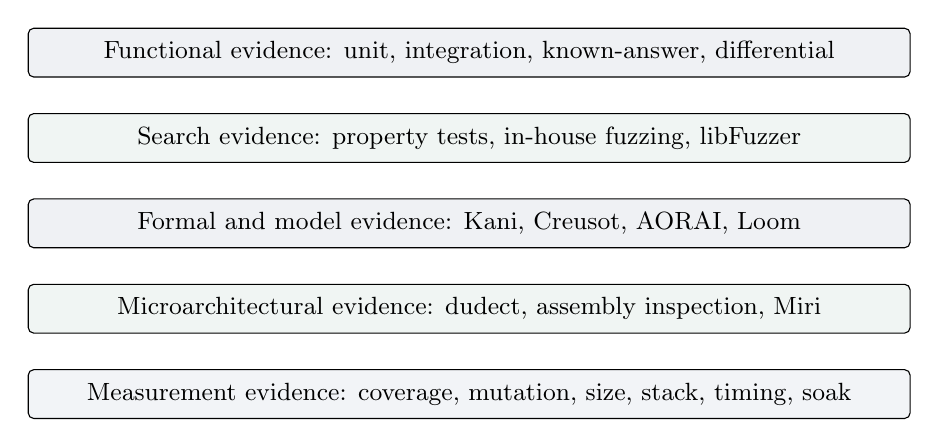
\begin{tikzpicture}[
  node distance=0.45cm,
  layer/.style={draw, rounded corners=2pt, minimum width=11.2cm, minimum height=0.62cm, align=center, font=\small},
  l1/.style={layer, fill=qwpblue!7},
  l2/.style={layer, fill=qwpgreen!7},
  l3/.style={layer, fill=qwpgray}
]
\node[l1] (a) {Functional evidence: unit, integration, known-answer, differential};
\node[l2, below=of a] (b) {Search evidence: property tests, in-house fuzzing, libFuzzer};
\node[l1, below=of b] (c) {Formal and model evidence: Kani, Creusot, AORAI, Loom};
\node[l2, below=of c] (d) {Microarchitectural evidence: dudect, assembly inspection, Miri};
\node[l3, below=of d] (e) {Measurement evidence: coverage, mutation, size, stack, timing, soak};
\end{tikzpicture}
\caption{The layered assurance model. Each layer answers a different question;
none is a substitute for an independent audit.}
\label{fig:assurance}
\end{figure}

\subsection{Tooling matrix}

\begin{table}[ht]
\centering
\caption{Verification and analysis tools, their role, and the latest measured
result. Tools marked unavailable are not installed.}
\label{tab:tools}
\footnotesize
\begin{tabularx}{\textwidth}{@{}>{\raggedright\arraybackslash}p{2.7cm}>{\raggedright\arraybackslash}p{2.0cm}Y>{\raggedright\arraybackslash}p{3.1cm}@{}}
\toprule
Tool & Version & Role & Latest result\\
\midrule
Kani & 0.68.0 & Parser and bounds model checking & 24 of 24 harnesses pass.\\
Creusot & 0.15.0-dev & Deductive arithmetic contracts & 7 of 7 contracts proved.\\
Frama-C AORAI & 33.0 & Temporal verification order on a C model & 1,050 of 1,051 goals; one typing timeout.\\
cargo-fuzz / libFuzzer & 0.13.2 & Coverage-guided fuzzing & 17,961,180 verifier runs; about 29 million per parser; no crash.\\
Proptest & 1.12 & Property-based testing & 5 properties, 64 cases each, plus 4 regressions.\\
Loom & 0.7.3 & Concurrency permutation model & Chunk-and-join model passes.\\
dudect-bencher & 0.7.0 & Statistical timing analysis & Valid paths at most 1.07 absolute t; control above 25,000.\\
cargo-show-asm & 0.2.64 & Assembly inspection & No secret-dependent indirect dispatch; no fence instructions.\\
Miri & nightly 2026-08-21 & Undefined-behavior checking & Classical 30 of 30; QHS-E guard 1 of 1.\\
cargo-llvm-cov & 0.9.1 & Source coverage & QHS-E 98.50 percent lines; 100 percent functions.\\
cargo-tarpaulin & 0.37.6 & Independent coverage engine & QHS-E 45 of 47 lines in the package run.\\
cargo-mutants & 27.1.0 & Mutation testing & Tables in this paper; all survivors classified.\\
Custom fuzz driver & in-tree & All-version robustness and soak & Per-version one-hour soaks pass.\\
Ferrocene & unavailable & Certified compiler path & Customer portal only; not installed.\\
\bottomrule
\end{tabularx}
\end{table}
\FloatBarrier

The tool matrix is deliberately mixed: no single tool is treated as a proof of
the whole system. The next subsections describe what each layer does and what it
does not do.

\subsection{Unit, integration, and known-answer tests}

The release suite contains 308 tests. It covers key generation, signing,
verification, parsing, serialization, caches, state guards, command-line
behavior, known-answer vectors, RFC 8032 Ed25519 vectors, and negative cases.
The tests are run in debug and release profiles. The release profile is the
one used for the evidence snapshot.

\subsection{Differential testing}

QHS-E is compared against the base verifiers for valid signatures, tampered
signatures, wrong messages, wrong keys, cross-version inputs, random
signatures, multiple leaves, and non-canonical public-key tails. The
differential suite is the main evidence for the equivalence lemma. The
exhaustive bit sweep and structural transplant suite extend the comparison to
every signature byte and to multi-byte structural substitutions.

\subsection{Property-based testing}

The proptest suite contains five properties with 64 cases each, plus four
regression tests. It checks that QHS-E accepts valid signatures and rejects
other messages, that every single-byte mutation of a valid signature is
rejected, that fixed and variable signature parsers round-trip, and that the
QHS-6 hybrid accepts its own signature and rejects an appended message. The
regression tests cover empty-message Ed25519, empty-message QHS-5, one-byte
QHS-6, and Ed25519 public-key round-trip.

\subsection{In-house fuzzing}

The deterministic fuzz driver exercises all versions in one process. It
generates random keys, messages, signatures, caches, and state files; it checks
round-trip behavior, parser behavior, and panic freedom. It accepts a seed and
prints progress every sixty seconds. The driver is the basis for the one-hour
and planned 72-hour soaks.

\subsection{libFuzzer}

Three libFuzzer targets cover the QHS-E verifier, the fixed and variable
signature parsers, and the QHS-6 hybrid parser. The QHS-E target uses canonical
headers and zero reserved tails for half of its inputs so that it reaches the
checksum, chain, and Merkle paths instead of stopping at the header. The latest
run completed 17,961,180 executions in 61 seconds with no crash. The parser
targets completed about 29 million executions each in 46 seconds.

\subsection{Kani}

Kani proves 24 parser and bounds harnesses across QHS-1, QHS-2, QHS-3,
QHS-3.1, QHS-4, QHS-4.2, QHS-5, and QHS-6. The harnesses cover fixed-layout
parsing, length checks, header checks, and index bounds. Kani is not used to
prove the full functional correctness of BLAKE3 or the complete verifier.

\subsection{Creusot}

Creusot proves seven contracts on a model of the QHS-E digit, checksum, and
Merkle arithmetic. The contracts state that base-64 digits stay below 64,
hexadecimal digits stay below 16, the checksum sums stay within their bounds,
the authentication-path offset stays below 384, and the leaf-index predicates
match the 256 and 4,096 bounds. The model is not a second production
implementation; it is a proof of the arithmetic that the production verifier
uses.

\subsection{AORAI and Frama-C}

AORAI, the temporal analysis plug-in of Frama-C, checks a C model of the QHS-E
verification order: parse header, check leaf index, check checksum, verify
chains, climb the Merkle path, accept. The run proves 1,050 of 1,051 goals; the
single timeout is a tool-generated typing precondition, not a temporal
property. AORAI analyzes C, not Rust, so the model is illustrative and the Rust
implementation is covered by the other layers.

\subsection{Loom}

Loom models the host parallel-leaf protocol: split a fixed array into disjoint
chunks, spawn one scoped worker per chunk, and join all workers. The model
checks that every index is written exactly once and is visible after join. The
production code has no shared mutable state; the model validates the chunk and
join protocol rather than a lock-based data structure.

\subsection{dudect and Welch timing}

The custom Welch harness measures signing and verification timing. The dudect
harness measures valid signatures with different Merkle leaf indices and a
positive control that compares a valid signature with an early checksum
rejection. The latest dudect run reports a maximum absolute t-value of about
1.07 on valid paths and a positive-control value above 25,000. The low valid
path values are consistent with no detectable timing separation on this host.
The positive control shows that the harness is sensitive.

\subsection{Assembly inspection}

cargo-show-asm is used to inspect the generated verifier functions. The
public entry points are inlined into the shared verifier body. The emitted
calls are direct or fixed indirect calls to named hash helpers. There is no
secret-dependent indirect dispatch in the verifier. No speculative-execution
fence instructions are emitted. The verifier operates on public data, and
LFENCE is x86-specific and not a general Spectre mitigation, so fences are not
injected; this is documented rather than silently omitted.

\subsection{Miri}

Miri checks the classical arithmetic and the QHS-E length guard for undefined
behavior. The classical suite passes 30 tests; the QHS-E guard passes one test.
The long differential tests are not run under Miri because BLAKE3 signing is
prohibitively slow in the interpreter.

\clearpage
\subsection{Coverage}

Coverage is measured with cargo-llvm-cov and independently with
cargo-tarpaulin. The llvm-cov numbers are authoritative because they include
the full test graph. QHS-E is at 98.50 percent line coverage and 100 percent
function coverage. The classical crate is at 99.67 percent lines and 100
percent functions. The remaining QHS-E lines are defensive branches that
cannot be reached through the fixed-size public API. Tarpaulin is used as a
second engine; its package-only numbers are lower because it instruments only
the selected package's tests.

\subsection{Mutation testing}

Mutation testing is used to check that the tests detect plausible code
changes. The project records the number of mutants, caught mutants, missed
mutants, and unviable mutants. Missed mutants are classified as equivalent or
non-equivalent. The QHS-E run tested 47 mutants, caught 46, and missed one
equivalent OR/XOR digit mutation. The classical field run tested 253 mutants,
caught 229, missed nine equivalent bit-packing mutations, and left 15
unviable. The classical scalar run tested 48 mutants, caught 40, missed three
equivalent mutations, and left five unviable. The qwp-crypto runs cover the
QHS-1, QHS-2, QHS-3, and QHS-6 source files; all missed mutants are documented
equivalents. The qwp-cli run tested 271 mutants, caught 241, missed 23, and
left 7 unviable. The missed set is dominated by diagnostic selftest return
values that still make the self-test command succeed, plus one equivalent
guard comparison. New unit tests cover the actionable state-guard and cache
authentication survivors; the recorded run predates those tests.

\subsection{Soak testing}

Each version has a one-hour soak on a pinned commit. The soak runs the
deterministic fuzz driver for exactly 3,600 seconds and checks for zero panics
and a zero exit status. QHS-1 passed with 793,945,578 iterations; the combined
QHS-1/2/3/3.1 soak passed with 360,181,413; QHS-4 passed with 91,191,782;
QHS-4.1 with 94,814,625; QHS-4.2 with 56,556,913; QHS-5 with 48,430,620;
QHS-6 with 36,957,000; QHS-E with 28,798,916. A 72-hour all-version runner is
prepared and smoke-tested but has not been run.

\subsection{Code size and stack}

The QHS-E static library is built for thumbv7em and riscv32imac with release
optimization, link-time optimization, one codegen unit, and abort-on-panic.
The measured text plus read-only data is 12,771 bytes on thumbv7em and 14,247
bytes on riscv32imac for all four verifier entry points. Stack frames are
measured with the nightly stack-size emission and read with llvm-readobj. The
peak verifier frame is about six kilobytes, driven by the BLAKE3 hasher; the
shared verifier frame is about 256 to 264 bytes. This is a fixed-size,
allocation-free profile, but it is not an eight-kilobyte-device profile.

\subsection{Toolchain and reproducibility}

The project builds with stable Rust 1.99 and uses a pinned nightly for Miri,
libFuzzer, and stack-size emission. Kani, cargo-fuzz, cargo-tarpaulin,
cargo-show-asm, Miri, Frama-C with AORAI, Alt-Ergo, Z3, opam, Why3, and
Creusot are installed. Ferrocene cannot be installed without a customer
account. The soak runner records the commit, binary hash, host, compiler
versions, seed, start and end times, and exit status. The evidence files record
the commands and raw outputs.

\section{Results}

\subsection{Release tests and attacks}

The release suite passes 308 tests with zero failures. The attack suite passes
20 of 20 groups. The full bit sweep flips every bit of every signature byte for
QHS-1, QHS-2, QHS-3, QHS-4, QHS-4.2, QHS-5, QHS-6, and the QHS-E verifier; no
mutation is accepted. The structural suite tampers with leaf indices, chain
values, authentication paths, forest entries, randomizers, and whole layers,
repairs the unkeyed checksum, and verifies; every case is rejected. The public
key mutation suite flips every public-key byte; parsing or verification
rejects. The cross-version suite feeds keys and signatures to the wrong
versions; all are rejected. The QHS-6 component suite mixes components across
messages and keys; all are rejected. The Ed25519 suite covers small-order
points, non-canonical scalars, identity nonces, and malleability; all are
rejected.

\subsection{Release and tag history}

\begin{table}[ht]
\centering
\caption{Version tags and the evidence snapshot. Earlier tags are preserved.}
\label{tab:tags}
\footnotesize
\begin{tabularx}{\textwidth}{@{}l l l Y@{}}
\toprule
Tag & Scope & Commit & Evidence\\
\midrule
qhs1-rc1 & QHS-1 & 6f398b0 & Proof, formats, tests, attacks, one-hour soak.\\
qhs2-rc1 & QHS-2 & 6f398b0 & Separate parameter set and evidence.\\
qhs3-rc1 & QHS-3 & 6f398b0 & Height-12 capacity and evidence.\\
qhs31-rc1 & QHS-3.1 & 6f398b0 & Same signature, tree cache.\\
qhs4-rc1 & QHS-4 & 035dbe2 & Stateless hypertree and forest; soak 91,191,782.\\
qhs41-rc1 & QHS-4.1 & 7177d1f & Parallel profile; soak 94,814,625.\\
qhs42-rc1 & QHS-4.2 & d50e9c8 & Compact stateless; soak 56,556,913.\\
qhs5-rc1 & QHS-5 & adea8db & 512-bit margin; soak 48,430,620.\\
qhs6-rc1 & QHS-6 & b0d2e39 & Hybrid; soak 36,957,000.\\
qhse-rc1 & QHS-E & 3a92256 & Verifier profile; soak 28,798,916.\\
\bottomrule
\end{tabularx}
\end{table}
\FloatBarrier

The main evidence snapshot used in this paper is commit 1bb413c. QHS-E
production code is identical to the tagged release; later commits add the
72-hour soak tooling, documentation, stack measurement, CLI guard and cache
tests, and this white paper. The 72-hour run will use a later commit with the
same production code.

\clearpage
\subsection{Attack catalogue}

\begin{table}[ht]
\centering
\caption{The twenty attack groups and the adversarial question each answers.}
\label{tab:attackcatalogue}
\footnotesize
\begin{tabularx}{\textwidth}{@{}>{\raggedright\arraybackslash}p{4.0cm}Y>{\raggedright\arraybackslash}p{2.4cm}@{}}
\toprule
Attack group & Question & Result\\
\midrule
Format and header attacks & Can version, algorithm, height, reserved, or leaf-index fields be confused? & Rejected.\\
Checksum repair & Does tampering survive when the unkeyed checksum is recomputed? & Rejected.\\
WOTS chain attacks & Can a chain value, chain end, or chain count be substituted? & Rejected.\\
Authentication-path attacks & Can a sibling, path level, or whole path be transplanted? & Rejected.\\
Whole-chunk transplants & Can WOTS, forest, or hypertree chunks be moved between positions? & Rejected.\\
Leaf-boundary attacks & Are zero, maximum, out-of-range, and overflow leaf indices handled? & Rejected.\\
Message-boundary attacks & Are empty, one-byte, block-boundary, and long messages handled? & Valid only for valid signatures.\\
Public-key mutation & Does every public-key byte affect parsing or verification? & Rejected after the tail fix.\\
Cross-version confusion & Can a key or signature be used under another version? & Rejected.\\
QHS-6 component mixing & Can QHS-5 or Ed25519 components be swapped across messages or keys? & Rejected.\\
QHS-6 embedded header & Is the embedded QHS-5 header canonical? & Rejected after the fix.\\
Ed25519 small order & Are identity and low-order points rejected? & Rejected.\\
Ed25519 non-canonical scalars & Are scalar values at or above the group order rejected? & Rejected.\\
Ed25519 nonce malleability & Is an identity or forged nonce rejected? & Rejected.\\
State guard corruption & Does a corrupt guard fail closed? & Refused.\\
State guard deletion & Does a missing guard for an advanced key fail closed? & Refused.\\
Rollback & Does a guard ahead of the key counter stop signing? & Refused.\\
Cache corruption and foreign cache & Does a bad cache fall back to recomputation? & Recomputed.\\
Full bit sweep & Does any single-bit signature change survive? & Zero accepted.\\
Differential verifier & Does QHS-E differ from the base verifier? & No divergence observed.\\
\bottomrule
\end{tabularx}
\end{table}
\FloatBarrier

\begin{table}[ht]
\centering
\caption{Attack and test summary.}
\label{tab:attacks}
\small
\begin{tabularx}{\textwidth}{@{}l Y r@{}}
\toprule
Evidence & Scope & Result\\
\midrule
Release tests & Workspace, debug and release & 308 pass, 0 fail\\
Attack groups & QHS family and QHS-E & 20 of 20 pass\\
Bit sweep & Every bit of every signature byte & 0 accepted\\
Structural checksum repair & Leaf, chain, path, forest, layer & 0 accepted\\
Public-key mutation & Every public-key byte & 0 accepted\\
Cross-version & QHS-1/2/3/4/4.2/5/6 & 0 accepted\\
QHS-6 component mixing & Messages, keys, headers & 0 accepted\\
Ed25519 edge cases & Small order, non-canonical, malleability & 0 accepted\\
\bottomrule
\end{tabularx}
\end{table}
\FloatBarrier

\subsection{Fuzz and soak results}

\begin{table}[ht]
\centering
\caption{Fuzz and soak evidence. The 72-hour run is prepared but not yet run.}
\label{tab:soak}
\small
\begin{tabularx}{\textwidth}{@{}l r r Y@{}}
\toprule
Run & Duration & Iterations & Result\\
\midrule
QHS-1 pre-soak & 1 hour & 793,945,578 & 0 panics\\
Combined QHS-1/2/3/3.1 & 1 hour & 360,181,413 & 0 panics\\
QHS-4 & 1 hour & 91,191,782 & 0 panics\\
QHS-4.1 & 1 hour & 94,814,625 & 0 panics\\
QHS-4.2 & 1 hour & 56,556,913 & 0 panics\\
QHS-5 & 1 hour & 48,430,620 & 0 panics\\
QHS-6 & 1 hour & 36,957,000 & 0 panics\\
QHS-E & 1 hour & 28,798,916 & 0 panics\\
All-version 72-hour runner & 72 hours & not yet run & prepared and smoke-tested\\
\bottomrule
\end{tabularx}
\end{table}
\FloatBarrier

\clearpage
\subsection{Coverage}

\begin{table}[ht]
\centering
\caption{Line and function coverage from the full llvm-cov test graph.}
\label{tab:coverage}
\small
\begin{tabularx}{\textwidth}{@{}l r r Y@{}}
\toprule
Target & Line coverage & Function coverage & Notes\\
\midrule
QHS-1 & 99.50 percent & 100 percent & Legacy 79.24 percent overall figure includes older containers.\\
QHS-2 & 99.35 percent & 100 percent & Full test graph.\\
QHS-3 & 99.17 percent & 100 percent & Full test graph.\\
QHS-4 & 99.28 percent & 100 percent & Full test graph.\\
QHS-4.1 & 99.28 percent & 100 percent & Same qhs4 source; platform signer tested byte-for-byte.\\
QHS-4.2 & 99.33 percent & 100 percent & Full test graph.\\
QHS-5 & 99.74 percent & 100 percent & Full test graph.\\
QHS-6 & 99.25 percent & 100 percent & Full test graph.\\
Classical crate & 99.67 percent & 100 percent & Field and scalar at 100 percent lines.\\
QHS-E & 98.50 percent & 100 percent & Three defensive branches remain.\\
\bottomrule
\end{tabularx}
\end{table}
\FloatBarrier

\clearpage
\subsection{Mutation}

\begin{table}[ht]
\centering
\caption{Mutation testing summary. Missed mutants are equivalent or documented.}
\label{tab:mutation}
\small
\begin{tabularx}{\textwidth}{@{}l r r r r Y@{}}
\toprule
Target & Tested & Caught & Missed & Unviable & Notes\\
\midrule
QHS-E & 47 & 46 & 1 & 0 & Equivalent OR/XOR digit mutation.\\
Classical field & 253 & 229 & 9 & 15 & Equivalent bit packing.\\
Classical scalar & 48 & 40 & 3 & 5 & Equivalent bit packing and dead carry.\\
QHS-1 source & 114 & 110 & 2 & 2 & Best-effort drop and equivalent root loop.\\
QHS-2 source & 119 & 113 & 3 & 3 & Drop, root loop, equivalent OR/XOR.\\
QHS-3 source & 165 & 131 & 7 & 27 & Drop, guard equivalents, OR/XOR; oversized-node test added.\\
QHS-6 source & 66 & 34 & 0 & 32 & No missed mutant.\\
QHS-core & 57 & 57 & 0 & 0 & All viable caught.\\
QHS-2 historical & 88 & 88 & 0 & 0 & Non-equivalent viable caught.\\
QHS-3/3.1 historical & 129 & 129 & 0 & 0 & Non-equivalent viable caught.\\
QHS-4 & 93 & 93 & 0 & 0 & Non-equivalent viable caught.\\
QHS-4.1 platform & 18 & 6 & 10 & 2 & Platform-only filter; one equivalent guard; other misses outside filter.\\
QHS-4.2 & 130 & 121 & 9 & 48 & Release-only paths and one best-effort drop.\\
QHS-5 & 94 & 91 & 3 & 32 & Best-effort drop and two equivalents.\\
QHS-6 historical & 64 & 32 & 32 & 0 & Profile split; see evidence file.\\
qwp-cli & 271 & 241 & 23 & 7 & Diagnostic selftest returns and one equivalent guard; new guard/cache tests added.\\
\bottomrule
\end{tabularx}
\end{table}
\FloatBarrier

\subsection{Performance and size}

\begin{table}[ht]
\centering
\caption{QHS-E embedded evidence.}
\label{tab:embedded}
\small
\begin{tabularx}{\textwidth}{@{}l r r Y@{}}
\toprule
Metric & thumbv7em & riscv32imac & Notes\\
\midrule
Code size & 12,771 B & 14,247 B & Text plus read-only data, all four entry points.\\
Peak verifier stack & about 6.0 KB & about 6.0 KB & BLAKE3 hasher frame.\\
Shared verifier frame & 264 B & 256 B & Excludes caller key and signature storage.\\
QHS-1 verification & 0.14 ms & host & Host measurement, not MCU cycles.\\
QHS-2 verification & 0.32 ms & host & Host measurement, not MCU cycles.\\
QHS-3/3.1 verification & 0.39 ms & host & Host measurement, not MCU cycles.\\
\bottomrule
\end{tabularx}
\end{table}
\FloatBarrier

\section{Operational Guidance}

\subsection{Choosing a version}

Use QHS-1 when signing speed and simplicity matter and the key can remain
stateful and single-writer. Use QHS-2 when signature size matters more than
signing speed. Use QHS-3 when a key must produce thousands of signatures; use
QHS-3.1 when signing latency matters and a host-side tree cache is acceptable.
Use QHS-4 when the signer cannot maintain a counter; use QHS-4.1 for faster
signing and QHS-4.2 for a smaller stateless signature. Use QHS-5 when a
256-bit classical margin is required. Use QHS-6 when a classical hybrid is
required for migration or compliance. Use QHS-E when the verifier is a
bootloader or constrained microcontroller.

\subsection{Stateful key lifecycle}

Generate the key on a trusted host. Keep the private key, cache, state guard,
and lock file private. Sign with a single writer. Back up the key and guard
together only if the backup is treated as a complete state snapshot; restoring
both to an older point reuses leaves. Never copy the key to a second signer.
Retire the key before the counter reaches its limit. Verify the state guard
after any crash or restore.

\subsection{Stateless signing}

QHS-4, QHS-4.1, and QHS-4.2 may be cloned and run concurrently. They have no
counter, cache, or state guard. The signer must still protect the private key
and must not reuse the same key material across different parameter sets.
Verification is stateless and can be parallelized.

\subsection{Embedded verifier}

QHS-E expects the caller to provide the exact public key and signature
buffers. It does not allocate, does not copy the full signature, and does not
use the heap. The caller must budget about six kilobytes of stack for the
verifier plus the key and signature storage. The verifier is public-data work;
timing differences on malformed inputs are not secret-dependent leaks.

\subsection{Backup and rollback}

The local state guard detects a guard that is ahead of the key counter, a
corrupt guard, and a missing guard for an advanced key. It cannot detect a
rollback of both the key and the guard, or a deletion of the guard combined
with a rollback to counter zero. Deployments that require stronger rollback
protection need an external trusted counter, a hardware security module, or an
append-only remote log.

\subsection{Migration to hybrid}

QHS-6 is the migration profile. It requires both the 512-bit-margin hash-based
signature and Ed25519. A deployment can accept QHS-6 while the classical
component remains trusted and retain the hash-based component if the classical
component is later weakened. The transcript binding prevents mixing components
from different messages or keys.

\section{Limitations and Assurance Gaps}

\subsection{No independent audit}

The largest gap is the absence of an independent cryptographic and
implementation audit. All proofs, tests, attacks, and measurements are
first-party. The project explicitly warns against using it for real security
without independent review.

\subsection{No certified compiler}

Ferrocene is distributed through a customer portal and requires an account and
token. The project builds with stable Rust 1.99 and has no ISO 26262 or
IEC 61508 certified compiler claim. This is an open gap for safety-critical
deployments.

\subsection{Coverage is not complete}

QHS-E is at 98.50 percent line coverage. The remaining lines are defensive
branches that cannot be reached through the fixed-size public API. The
classical crate is at 99.67 percent. The project does not claim complete path
execution.

\subsection{Formal verification is partial}

Kani proves parser and bounds properties. Creusot proves an arithmetic model.
AORAI checks a C model of the verification order. None of these proves the
full Rust verifier together with BLAKE3 end to end. A full proof would require
a verified hash implementation or a much larger model.

\subsection{Stack budget}

QHS-E's peak verifier frame is about six kilobytes. This is fixed and
allocation-free, but it is not suitable for very small microcontrollers with
only a few kilobytes of RAM. The caller must budget for the verifier plus the
key and signature storage.

\subsection{State guard residual}

The state guard is local software. It cannot detect a rollback of both the key
and the guard, or a guard deletion combined with a rollback to counter zero.
Deployments that need stronger protection must add external trusted state.

\subsection{Speculative-execution fences}

No speculative-execution fence instructions are injected. The verifier handles
public data and has no secret-dependent memory access. LFENCE is
x86-specific and is not a general Spectre mitigation. The decision is
documented and the assembly is inspected.

\subsection{Research backlog}

The braid reduction, the Temperley--Lieb solver, and the braid cryptanalysis
items remain research backlog. They are not production signature paths and are
not part of the release claims.

\clearpage
\subsection{Residual gap matrix}

\begin{table}[ht]
\centering
\caption{Residual assurance gaps and limitations. These are not hidden by the
empty production gap register.}
\label{tab:residual}
\footnotesize
\begin{tabularx}{\textwidth}{@{}>{\raggedright\arraybackslash}p{3.7cm}>{\raggedright\arraybackslash}p{2.2cm}Y@{}}
\toprule
Gap & Status & Consequence\\
\midrule
Independent audit & Open & The project is not externally reviewed.\\
Certified compiler & Open & No ISO 26262 or IEC 61508 compiler claim.\\
Complete path coverage & Open & QHS-E 98.50 percent; classical 99.67 percent.\\
Full formal proof & Partial & Parser, bounds, and arithmetic model only.\\
Embedded stack & Limitation & About six kilobytes peak verifier frame.\\
State guard at counter zero & Residual & Rollback of both key and guard is not detectable.\\
Speculative-execution fences & Not applied & Public-data verifier; LFENCE is not portable.\\
72-hour soak & Prepared, not run & The runner and plan exist; the run is pending.\\
qwp-cli mutation & Completed & Diagnostic and equivalent survivors; guard/cache tests added.\\
QHS-1 72-hour soak & Waived & Only the one-hour soak is claimed.\\
\bottomrule
\end{tabularx}
\end{table}
\FloatBarrier

\section{Future Work}

The next steps are external, not more local tests:

\begin{enumerate}
  \item Run the prepared 72-hour all-version soak on an idle machine.
  \item Commission an independent cryptographic and implementation audit.
  \item Evaluate a certified compiler path, such as Ferrocene, under the
  appropriate license.
  \item Extend formal verification toward the full verifier and the hash
  function, or clearly bound the verified core.
  \item Measure cycles and stack on real microcontroller hardware.
  \item Add external trusted state for deployments that require stronger
  rollback protection.
  \item Publish a stable release package with reproducible builds and a
  complete evidence bundle.
\end{enumerate}

\section{Conclusion}

\qwp{} is a deliberately conservative hash-based signature family with a
small dependency graph, a strict code standard, explicit version separation,
and an unusually broad local verification programme. The family covers
stateful and stateless signing, compact and high-capacity profiles, a 512-bit
margin, a classical hybrid, and an embedded verifier. The evidence is strong
for a first-party project: 308 release tests, 20 attack groups, an exhaustive
bit sweep with no accepted mutation, model checking, deductive verification,
temporal analysis, concurrency modeling, timing analysis, assembly inspection,
undefined-behavior checking, coverage, mutation testing, code-size and stack
measurement, and per-version one-hour soaks. QHS-E passed its soak and is
tagged.

The project is not externally audited and is not a standard. The remaining
gaps are assurance gaps, not missing local test cases. The correct next step is
to freeze the internal evidence, run the prepared 72-hour soak, and hand the
bundle to an independent reviewer.

\appendix

\section{Version parameter details}

\begin{longtable}{@{}>{\raggedright\arraybackslash}p{2.0cm}>{\raggedright\arraybackslash}p{4.0cm}>{\raggedright\arraybackslash}p{4.0cm}>{\raggedright\arraybackslash}p{4.2cm}@{}}
\caption{Detailed parameter comparison.}\\
\toprule
Version & One-time signature & Tree or hypertree & Encoding and notes\\
\midrule
\endfirsthead
\toprule
Version & One-time signature & Tree or hypertree & Encoding and notes\\
\midrule
\endhead
QHS-1 & 67 chains, 15 steps, 32-byte values & Merkle height 8, 256 leaves & 64 hex digits plus 3 checksum digits; 64-byte keys.\\
QHS-2 & 45 chains, 63 steps, 32-byte values & Merkle height 8, 256 leaves & 43 base-64 digits plus 2 checksum digits; 64-byte keys.\\
QHS-3 & 45 chains, 63 steps, 32-byte values & Merkle height 12, 4,096 leaves & 43 base-64 digits plus 2 checksum digits; 384-byte path.\\
QHS-3.1 & Same as QHS-3 & Same as QHS-3 & Tree cache for fast signing; same signatures.\\
QHS-4 & 45 chains, 63 steps, 32-byte values & Eight layers of height 8; forest 16 by 8 & 68-byte keys; stateless; 18,216-byte signature.\\
QHS-4.1 & Same as QHS-4 & Same as QHS-4 & Parallel tree and forest generation; byte-identical signatures.\\
QHS-4.2 & 34 chains, 255 steps, 32-byte values & Seven layers of height 8; forest 17 by 8 & 68-byte keys; stateless; 14,344-byte signature.\\
QHS-5 & 89 chains, 63 steps, 64-byte values & Merkle height 8, 256 leaves & 86 base-64 digits plus 3 checksum digits; 72-byte keys; 512-bit hash.\\
QHS-6 & QHS-5 plus Ed25519 & QHS-5 tree & Transcript-bound hybrid; 108-byte keys; 6,284-byte signature.\\
QHS-E & Verifier-only & Base version & Same keys and signatures; no signing or state.\\
\bottomrule
\end{longtable}

\section{Evidence inventory}

The evidence bundle contains the following categories. Each file records the
command, date, scope, raw output, and result.

\begin{itemize}
  \item Per-version attack-suite and fuzz results.
  \item Per-version one-hour soak logs and the QHS-E soak log.
  \item Coverage reports for QHS-1 through QHS-6, the classical crate, and
  QHS-E.
  \item Mutation reports for the core, crypto, classical, QHS-E, platform, and
  CLI crates.
  \item Kani harness summaries for the proof crate.
  \item Creusot, AORAI, Loom, dudect, Miri, tarpaulin, and assembly evidence
  for the verification tooling.
  \item Code-size and stack evidence for the embedded profile.
  \item The 72-hour soak plan and the smoke-test log.
  \item The code-standard audit and the break log.
\end{itemize}

\section{Glossary}

\begin{description}[style=nextline]
  \item[Authentication path] The sibling hashes needed to climb from a leaf to
  the Merkle root.
  \item[Chain] A sequence of hash applications in a Winternitz one-time
  signature.
  \item[Checksum] A small unkeyed value used for corruption detection; it is
  not an authenticator.
  \item[FORS] A forest of few-time signatures used by the stateless versions.
  \item[Hypertree] A multi-layer tree that lets a stateless signer authenticate
  fresh subtrees.
  \item[Leaf] A one-time public key at the bottom of a Merkle tree.
  \item[State guard] A keyed local record used to detect some rollback cases.
  \item[Transcript] The key-and-message string signed by both components of the
  hybrid.
  \item[WOTS] A Winternitz one-time signature built from hash chains.
\end{description}

\section{Code-standard lint inventory}

\begin{longtable}{@{}>{\raggedright\arraybackslash}p{3.4cm}>{\raggedright\arraybackslash}p{8.0cm}>{\raggedright\arraybackslash}p{3.4cm}@{}}
\caption{Detailed lint inventory by purpose. The names are compiler lint
families; the paper does not reproduce source attributes.}\\
\toprule
Category & Controls & Intent\\
\midrule
\endfirsthead
\toprule
Category & Controls & Intent\\
\midrule
\endhead
Default patterns & all, pedantic, nursery, cargo & Catch broad accidental complexity, suspicious conversions, undocumented behavior, and packaging mistakes.\\
Core isolation & alloc\_instead\_of\_core, std\_instead\_of\_core, std\_instead\_of\_alloc & Prevent accidental reliance on allocation or the standard library in the cryptographic core.\\
Panic matrix & unwrap\_used, expect\_used, indexing\_slicing, panic, todo, unimplemented, unreachable & Remove compiled crash branches and unchecked fixed-array access.\\
Casts and side channels & as\_conversions, cast\_lossless, cast\_possible\_truncation, cast\_possible\_wrap, float\_arithmetic & Force explicit bounded conversions and remove floating-point non-determinism.\\
Compiler shape & missing\_inline\_in\_public\_items, exhaustive\_structs, exhaustive\_enums & Make public API boundaries explicit and prevent silent field or variant addition.\\
Additional hardening & arithmetic\_side\_effects, panic\_in\_result\_fn, unwrap\_in\_result, allow\_attributes\_without\_reason, dbg\_macro, exit, mem\_forget, print\_stdout, print\_stderr, let\_underscore\_must\_use, missing\_debug\_implementations, missing\_docs, rustdoc::all, unreachable\_pub, unused\_results, let\_underscore\_drop, non\_ascii\_idents, rust\_2018\_idioms, future\_incompatible, trivial\_casts, trivial\_numeric\_casts, unused\_qualifications, unused\_lifetimes, single\_use\_lifetimes, elided\_lifetimes\_in\_paths & Close the remaining panic, side-effect, documentation, visibility, and lifetime gaps.\\
\bottomrule
\end{longtable}

The production crypto crates apply the full set. The classical crate keeps
style-only exceptions for conventional single-letter names, grouped field
literals, explicit internal visibility, and cargo metadata; it does not keep an
indexing, cast, or unchecked-arithmetic exception. Host adapters apply the
security lints but allow standard-library use, terminal output, and test
assertions with reasons. The proof and size crates are evidence profiles, not
shipping libraries.

\begin{thebibliography}{99}

\bibitem{blake3}
J. O'Connor, J.-P. Aumasson, S. Neves, and Z. Wilcox-O'Hearn.
\newblock BLAKE3: one function, fast everywhere.
\newblock Specification and reference implementation, 2020.

\bibitem{rfc8032}
S. Josefsson and I. Liusvaara.
\newblock Edwards-Curve Digital Signature Algorithm (EdDSA).
\newblock RFC 8032, 2017.

\bibitem{fips180}
National Institute of Standards and Technology.
\newblock Secure Hash Standard (SHS).
\newblock FIPS 180-4, 2015.

\bibitem{fips202}
National Institute of Standards and Technology.
\newblock SHA-3 Standard: Permutation-Based Hash and Extendable-Output
Functions.
\newblock FIPS 202, 2015.

\bibitem{sp800208}
National Institute of Standards and Technology.
\newblock Recommendation for Stateful Hash-Based Signature Schemes.
\newblock NIST Special Publication 800-208, 2020.

\bibitem{rfc8554}
D. McGrew, M. Curcio, and S. Fluhrer.
\newblock Leighton-Micali Hash-Based Signatures.
\newblock RFC 8554, 2019.

\bibitem{merkle}
R. C. Merkle.
\newblock A certified digital signature.
\newblock In Advances in Cryptology, 1989.

\bibitem{kani}
Kani Rust Verifier.
\newblock Model checking for Rust.
\newblock Project documentation and tooling, 2026.

\bibitem{creusot}
Creusot.
\newblock Deductive verification for Rust.
\newblock Project documentation and tooling, 2026.

\bibitem{frama}
Frama-C and AORAI.
\newblock Temporal verification of C programs.
\newblock Project documentation and tooling, 2026.

\bibitem{dudect}
O. Reparaz, J. Balasch, and B. Gierlichs.
\newblock Dude, is my code constant time?
\newblock IACR ePrint 2016/1123.

\bibitem{loom}
Loom.
\newblock Permutation testing for concurrent Rust code.
\newblock Project documentation and tooling, 2026.

\bibitem{libfuzzer}
LLVM Project.
\newblock libFuzzer: a library for coverage-guided fuzz testing.
\newblock LLVM documentation, 2026.

\bibitem{miri}
Rust Project.
\newblock Miri: an interpreter for Rust's mid-level intermediate
representation.
\newblock Project documentation, 2026.

\bibitem{cargomutants}
cargo-mutants.
\newblock Mutation testing for Rust.
\newblock Project documentation and tooling, 2026.

\bibitem{llvmcov}
LLVM Project.
\newblock Source-based code coverage.
\newblock LLVM documentation, 2026.

\bibitem{ferrocene}
Ferrocene.
\newblock A qualified Rust toolchain for safety-critical systems.
\newblock Project documentation, 2026.

\bibitem{iso26262}
International Organization for Standardization.
\newblock ISO 26262: Road vehicles --- Functional safety.
\newblock Standard, 2018.

\bibitem{iec61508}
International Electrotechnical Commission.
\newblock IEC 61508: Functional safety of electrical/electronic/programmable
electronic safety-related systems.
\newblock Standard, 2010.

\bibitem{qwp}
\qwp{} Project.
\newblock Internal architecture decisions, proofs, formats, evidence, code
standard audit, gap register, break log, and traceability matrix.
\newblock Local documentation snapshot, 2026.

\end{thebibliography}

\end{document}
